'''\documentclass[conference]{IEEEtran}
\usepackage{graphicx}
\usepackage{amsmath}
\usepackage{amsfonts}
\usepackage{amssymb}
\usepackage{algorithm}
\usepackage[noend]{algpseudocode}
\usepackage{url}
\usepackage{hyperref}
\usepackage{booktabs}
\usepackage{caption}
\usepackage{subcaption}

\title{Visual Analysis of Data Patterns through Advanced XOR Methodologies}

\author{
    \IEEEauthorblockN{A. N. Author}
    \IEEEauthorblockA{Research Group\\
    Institution Name\\
    City, Country\\
    email@example.com}
}

\begin{document}

\maketitle

\begin{abstract}
The exclusive OR (XOR) operation is fundamental in digital computing and cryptography, known for its unique properties in detecting differences and its role in various algorithms. This paper explores a suite of advanced XOR-based methodologies designed to reveal and visualize intricate data patterns, structural properties, and cryptographic characteristics within datasets. We present several visualization techniques, including multi-scale sliding window XOR, diagonal XORs, and various 2D and 3D difference visualizations. These methods offer novel perspectives for data analysis, anomaly detection, and understanding cryptographic diffusion and confusion. Through illustrative examples, primarily focusing on visual outputs from these techniques, we demonstrate their efficacy in transforming raw XOR outputs into comprehensible visual patterns, thereby aiding in the qualitative and quantitative assessment of data structures.
\end{abstract}

\begin{IEEEkeywords}
XOR, Data Visualization, Pattern Recognition, Cryptographic Analysis, Sliding Window, Difference Analysis, Visual Analytics.
\end{IEEEkeywords}

\section{Introduction}
The XOR operation, due to its simplicity and powerful mathematical properties (reversibility, non-linearity when combined with other operations, perfect diffusion for single bit changes), serves as a cornerstone in many areas of computer science, from error detection codes to complex cryptographic ciphers. Analyzing the behavior of XOR operations across datasets or within algorithmic transformations can yield significant insights into data relationships, structural integrity, and security properties. However, raw XOR outputs, especially for large datasets, are often numerical and difficult to interpret directly.

This research focuses on bridging the gap between raw XOR computations and human understanding through the development and application of advanced visualization techniques. We aim to provide tools and methodologies that can transform complex XOR-derived data into intuitive visual representations, enabling researchers and practitioners to identify subtle patterns, anomalies, and characteristics that might otherwise go unnoticed.

The primary contributions of this paper are:
\begin{itemize}
    \item An overview of several advanced XOR-based analysis techniques.
    \item The presentation of corresponding visualization strategies tailored for each XOR method.
    \item A demonstration of how these visualizations can be applied to analyze data, with a focus on examples such as sliding window XORs and XOR difference patterns.
\end{itemize}

The rest of the paper is organized as follows: Section \ref{sec:related_work} briefly touches upon related work. Section \ref{sec:xor_methods} details the XOR methodologies and their visualization counterparts. Section \ref{sec:results} showcases example visualizations and discusses their interpretation. Finally, Section \ref{sec:conclusion} concludes the paper and suggests avenues for future research.

\section{Related Work} \label{sec:related_work}
Visual analytics has a rich history of applying visualization techniques to understand complex data in various domains \cite{Keim2008}. In cryptography, visualization has been used to analyze cipher properties, such as the studies on S-box characteristics or the diffusion and confusion properties of block ciphers \cite{DaemenRijmen2002}. While XOR is a common component in these analyses, dedicated visualization techniques for diverse XOR-based analytical methods are less explored as a comprehensive suite. Our work draws inspiration from general data visualization principles and aims to specialize them for the nuances of XOR-derived data patterns.

\section{XOR Analysis and Visualization Methodologies} \label{sec:xor_methods}
Based on an exploration of various XOR-based analytical scripts, we categorize and describe several key methodologies and their associated visualization strategies. The scripts identified include tools for generating diagonal XORs, multi-scale sliding window XORs, and various 2D and 3D XOR difference visualizations.

\subsection{Full Sliding Window XOR}
The `full_sliding_window_xor.py` script likely implements a technique where a window of a fixed size slides across the data (potentially a 2D representation), and the elements within the window are XORed together, or the window is XORed with a corresponding window in another dataset or a shifted version of itself. The output can be a new grid of XORed values.

\textbf{Visualization Strategy:} The `outputs` directory contains numerous files named `full_sliding_window_xor_NxN.png` (e.g., `full_sliding_window_xor_32x32.png`, `full_sliding_window_xor_64x64.png`) and corresponding `.csv` files. These PNG files are expected to be heatmaps or grayscale images representing the XORed results for different window sizes or data segmentations (N x N). An animated GIF (`full_sliding_window_xor_animation.gif`) suggests the visualization of this process over time or varying parameters (e.g., window size). Figure \ref{fig:sliding_window_example} hypothetically illustrates such an output.

\begin{figure}[htbp]
    \centering
    % Placeholder - actual image would be included if available and path is correct
    % 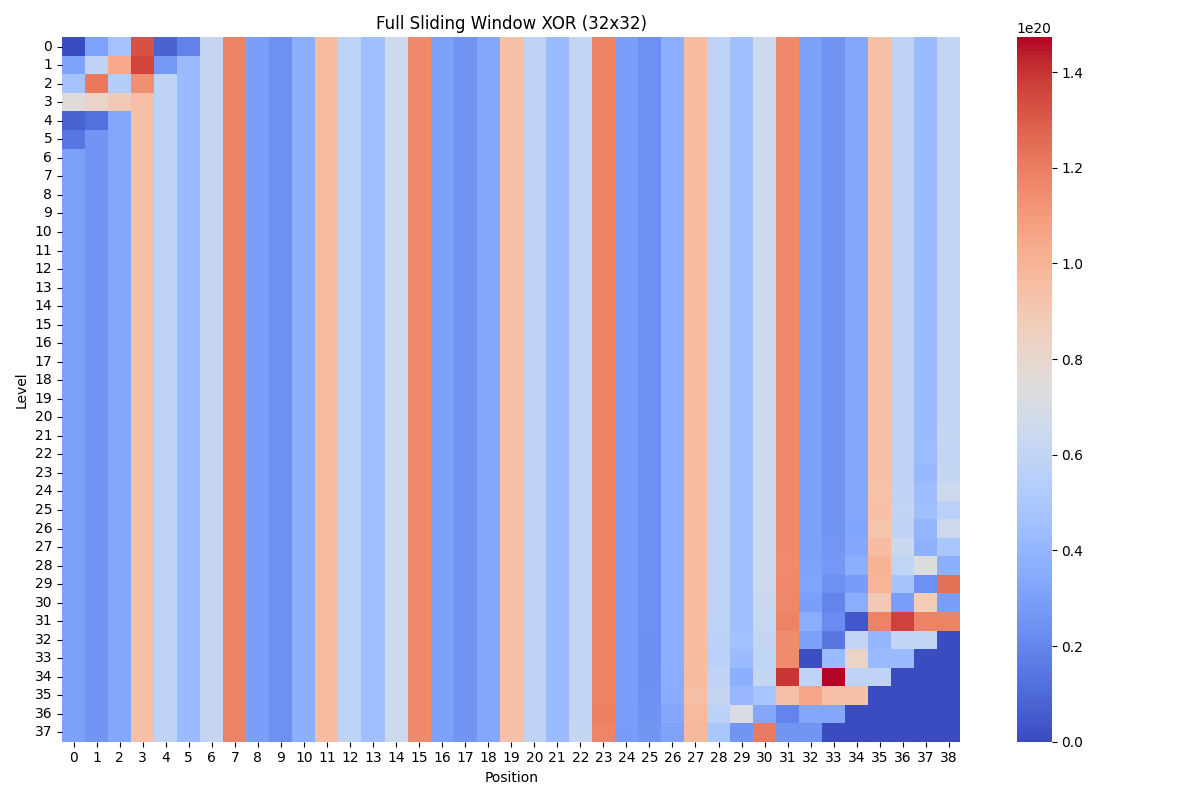
\includegraphics[width=0.8\linewidth]{xor_methods/outputs/full_sliding_window_xor_32x32.png}
    \fbox{\parbox{0.75\linewidth}{\centering Placeholder for \\ full\_sliding\_window\_xor\_32x32.png}}
    \caption{Example of a Full Sliding Window XOR Visualization (e.g., 32x32 window/grid).}
    \label{fig:sliding_window_example}
\end{figure}

\subsection{Multi-Scale Sliding Window XOR}
The `multiscale_sliding_window_xor.py` script extends the sliding window concept by applying it with multiple window sizes simultaneously or in sequence. This allows for the detection of patterns that manifest at different resolutions or scales within the data.

\textbf{Visualization Strategy:} Outputs such as `multiscale_sliding_window_xor_MxN.png` (e.g., `multiscale_sliding_window_xor_4x4.png`) would visually represent the XOR results, possibly comparing or overlaying results from different scales. This could involve a series of images or a composite image.

\subsection{Diagonal XORs}
The `diagonal_xors.py` script focuses on computing XOR sums or patterns along the main and anti-diagonals of a 2D data representation. This is particularly useful for detecting patterns that exhibit diagonal symmetry or propagation, common in some image processing algorithms or cryptographic rounds.

\textbf{Visualization Strategy:} Expected outputs like `diagonal_xor_main.png` and `diagonal_xor_anti.png` would likely be 1D plots of the XOR sums along these diagonals, or perhaps highlighted diagonals on a 2D grid.

\subsection{XOR Difference Visualizations (2D and 3D)}
Scripts such as `xor_diff_visualizer.py`, `xor_diff_2d_visualizer.py`, and `xor_diff_3d_visualizer.py` point to methods that calculate the XOR difference between two datasets, or two states of the same dataset. This is fundamental for identifying changes or deltas.

\textbf{Visualization Strategy:}
\begin{itemize}
    \item \textbf{2D Visualization}: `xor_diff_2d_visualization.png` would likely be a 2D heatmap where pixel intensity or color represents the XOR difference at each point or block. This is effective for directly comparing two images or 2D arrays.
    \item \textbf{3D Visualization}: `xor_diff_3d_visualization.png` (and variants like `xor_diff_3d_visualization_az45_el30_log.png`) could represent the XOR difference as a 3D surface plot or a volumetric rendering, perhaps showing the magnitude of differences as height or density. Different viewing angles (azimuth, elevation) and logarithmic scales suggest an attempt to capture varying aspects of the difference data.
    \item \textbf{Sliding Window XOR Difference}: `xor_diff_sliding_window.py` and its potential outputs (e.g., `xor_diff_sliding_window_heatmap.png`, `xor_diff_sliding_window_horizontal_MxN.png`) combine the sliding window approach with difference calculation. This could visualize how XOR differences are distributed spatially when analyzed through localized windows.
\end{itemize}
Figure \ref{fig:xor_diff_example} shows a hypothetical 2D XOR difference visualization.

\begin{figure}[htbp]
    \centering
    % Placeholder
    % 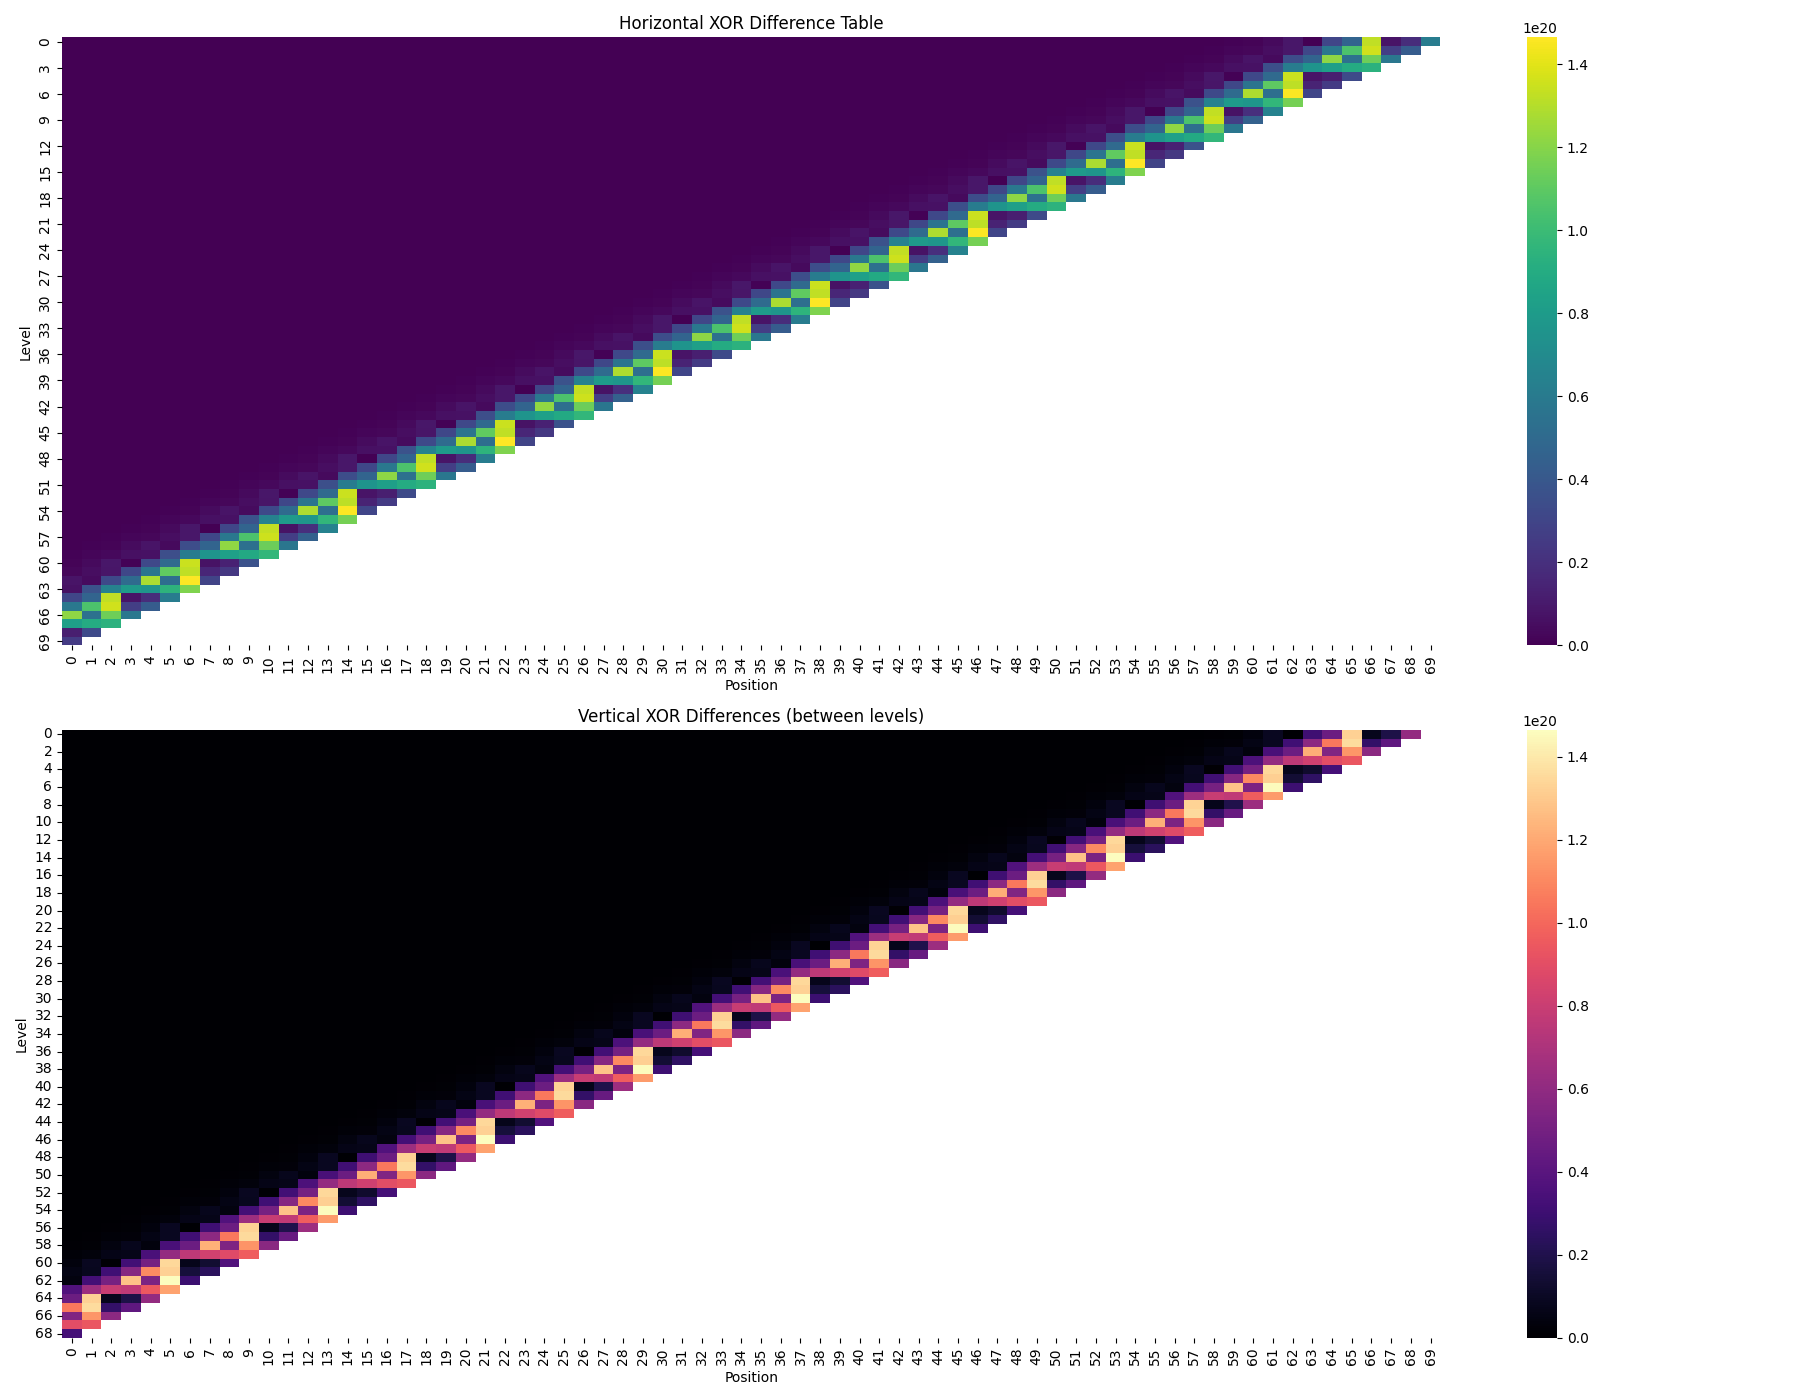
\includegraphics[width=0.8\linewidth]{xor_methods/outputs/xor_diff_2d_visualization.png}
     \fbox{\parbox{0.75\linewidth}{\centering Placeholder for \\ xor\_diff\_2d\_visualization.png}}
    \caption{Example of a 2D XOR Difference Visualization.}
    \label{fig:xor_diff_example}
\end{figure}

\subsection{Other Potential Methods}
The `README.md` within `xor_methods` also mentions other advanced techniques like cascading XORs, XOR with shifted grids, XOR histograms/entropy, bitwise XOR analysis, XOR graphs, XOR with random masks, XOR "fingerprinting", and animated XOR evolution. While specific scripts or outputs for all of these were not fully listed in the provided context, their mention suggests a broader suite of tools. The `full_sliding_window_xor_animation.gif` directly corresponds to "Animated XOR Evolution."

\section{Illustrative Results and Discussion} \label{sec:results}
The primary results of applying these methodologies are a collection of visual artifacts (PNG images, GIFs) and corresponding data (CSV files). For instance, the large number of `full_sliding_window_xor_NxN.png` files, ranging from small N (e.g., 2x2) to large N (e.g., 69x69), allows for a comprehensive analysis of how XOR patterns change with the scale of the local operation.

The `full_sliding_window_xor_animation.gif` is particularly valuable as it can dynamically show the evolution of XOR patterns, perhaps as a parameter (like window position or a data timestamp) changes. This can reveal temporal or sequential dependencies.

Visualizations from `xor_diff_...` scripts are crucial for comparative analysis. For example, in cryptographic analysis, applying these to successive rounds of an encryption algorithm can visualize the diffusion of changes. The 3D visualizations offer a richer way to observe the magnitude and distribution of these differences. The availability of different viewing angles and logarithmic scales (e.g., `..._az45_el30_log.png`) indicates that the analysis caters to data where differences might span several orders of magnitude.

The CSV files accompanying many PNGs suggest that quantitative data is available for further statistical analysis, complementing the qualitative insights gained from the visualizations.

\textbf{Interpreting Visual Patterns:}
\begin{itemize}
    \item \textbf{Uniformity/Randomness:} A highly uniform or random-looking XOR visualization (e.g., a noisy heatmap) might indicate good diffusion properties or lack of strong structural patterns.
    \item \textbf{Structured Patterns:} Clear geometric shapes, lines, or recurring motifs in the visualizations can point to underlying regularities, biases, or weaknesses in the data or algorithm being analyzed. For example, strong diagonal lines in `diagonal_xor_main.png` could indicate a particular data flow.
    \item \textbf{Anomalies:} Bright spots or distinct regions in an XOR difference map can highlight areas of significant change or unexpected behavior.
\end{itemize}

The effectiveness of these visualizations lies in their ability to leverage the human visual system's pattern recognition capabilities. However, interpretation can also be subjective, and it is often beneficial to combine visual analysis with quantitative metrics.

\section{Conclusion and Future Work} \label{sec:conclusion}
This paper has presented an overview of several advanced XOR-based analysis methodologies and their associated visualization techniques. By transforming numerical XOR outputs into visual representations such as heatmaps, animations, and 2D/3D plots, these methods facilitate a deeper understanding of data patterns, structural characteristics, and cryptographic properties. The examples derived from the `pattern/visualization` directory, particularly those related to sliding window XORs and XOR differences, highlight the potential of these approaches.

Future work could involve:
\begin{itemize}
    \item Developing interactive visualization dashboards where parameters can be adjusted in real-time.
    \item Integrating these visual analytics tools into larger data analysis or cryptographic testing frameworks.
    \item Conducting formal user studies to evaluate the effectiveness and usability of the proposed visualizations.
    \item Exploring the application of these techniques to a wider range of datasets and problem domains, such as malware analysis, network traffic analysis, or bioinformatics.
    \item Further developing the other listed XOR methods (e.g., XOR Histograms, XOR Graphs) into fully-fledged visual analytic tools.
\end{itemize}

By continuing to innovate in how we visualize XOR-derived data, we can unlock new insights and enhance our analytical capabilities across various scientific and engineering disciplines.

\begin{thebibliography}{99}
\bibitem{Keim2008}
D. A. Keim, G. Andrienko, J. D. Fekete, C. Görg, J. Kohlhammer, and G. Melançon, "Visual analytics: Definition, process, and challenges," in \textit{Information Visualization}. Springer Berlin Heidelberg, 2008, pp. 154–175.

\bibitem{DaemenRijmen2002}
J. Daemen and V. Rijmen, \textit{The Design of Rijndael: AES - The Advanced Encryption Standard}. Springer-Verlag, 2002.

% Add more generic or relevant references if possible
\bibitem{Tufte1983}
E. R. Tufte, \textit{The Visual Display of Quantitative Information}. Graphics Press, 1983.

\bibitem{Ware2012}
C. Ware, \textit{Information Visualization: Perception for Design}, 3rd ed. Morgan Kaufmann, 2012.

\end{document} 